% latexmk -shell-escape -pvc slides.tex # Watches and compiles on each change.
% latexmk -c slides.tex   # Clean the temporal files.

% NOTE: Slides explaining bibliometrix figures:
% https://bibliometrix.org/biblioshiny/assets/player/KeynoteDHTMLPlayer.html#109

\documentclass[aspectratio=169]{beamer}

\setbeamertemplate{footline}[frame number]

\usepackage{hyperref}
\usepackage{caption}
\usepackage{siunitx}
\usepackage{minted}
\usepackage[numbers]{natbib}
\usepackage{subcaption}
\usepackage{graphicx}

\captionsetup[figure]{labelformat=empty}

\newmintedfile[inputsql]{sql}{%
    linenos,
    autogobble,
    breaklines,
}


\title{Bibliometric analysis of TreesLab scientific production}

\author{Alber S\'{a}nchez \href{mailto:alber.ipia@inpe.br}
{alber.ipia@inpe.br} \\ 
Guilherme Mataveli \href{mailto:guilherme.mataveli@inpe.br}
{guilherme.mataveli@inpe.br}}
\institute{
  
\includegraphics[width=4cm,keepaspectratio]{logos/trees-color-h_2.png}
  
\includegraphics[width=1.8cm,keepaspectratio]
  {logos/logoinpe-azul-menor.png} \\
  Research assistant - TreesLab\\National Institute for Space Research - INPE\\
  Brazil
}
\date{\today}

\begin{document}

\frame{\titlepage}

\begin{frame}
  \frametitle{Overview} 
  \tableofcontents
\end{frame}


\section{Introduction}

\begin{frame}
  \frametitle{Introduction}
  \begin{itemize}
    \item Most of the definitions in this presentation were taken from 
      \citeauthor{aria2017} or any of their papers, webpages, tutorials, or 
      videos.
    \item We assumed that TreesLab's papers are an study subject.
  \end{itemize}
\end{frame}

% \begin{frame}
%   \frametitle{What is bibliometry?}
% \end{frame}

\begin{frame}
  \frametitle{Bibliometrix package}
  \begin{itemize}
    \item R package for bibliometric analysis~\cite{aria2017}. 
    \item It allows quantitative research in bibliometrics and scientometrics.
    \item Statistical analysis of publications.
    \item Useful for performance evaluation and policy making.
  \end{itemize}
\end{frame}

\begin{frame}
  \frametitle{Bibliometrix}
  \begin{itemize}
    \item Import and convert data from bibliographic databases.
    \item Analysis of a publication dataset.
    \item Building matrices of co-citation, coupling, collaboration, and 
      co-word analysis.
  \end{itemize}
\end{frame}

\begin{frame}
  \frametitle{Bibliographic databases}
  \begin{itemize}
    \item \href{https://www.scopus.com}{Scopus}. 
    \item \href{https://www.webofknowledge.com}{Web of science}.
    \item To query them, use a machine at INPE and your Café login.
  \end{itemize}
\end{frame}



\section{Method}

\begin{frame}
  \frametitle{Data pre-processing}
  \begin{enumerate}
    \item Retrieve DOI from TreesLab publication's webpage. 
    \item Query Scopus .
    \item Query Web of Science.
    \item Merge query results (Bibliometrix).
    \item Run analysis .
      \begin{itemize}
        \item Bibliometrix: R coders.
        \item Biblioshiny: Non-coders.
      \end{itemize}
  \end{enumerate}
\end{frame}



\section{Data analysis}

\subsection{Overview}

\begin{frame}
  \frametitle{Main information}
  \begin{figure}
    \centering
    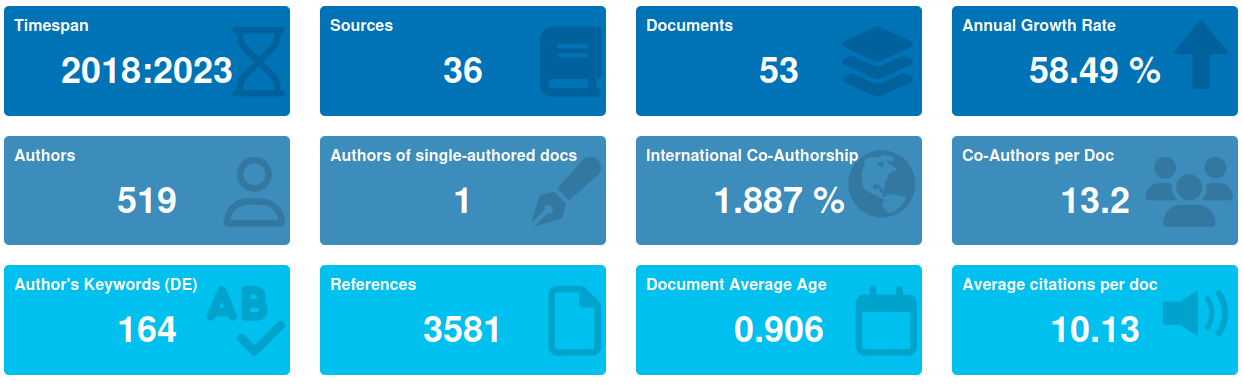
\includegraphics[width=0.8\textwidth]{img/main_information.png}
    %\caption{Main information about the bibliographic collection.}
    \label{fig:main_information}
  \end{figure}
\end{frame}

\begin{frame}
  \frametitle{Annual scientific production}
  \begin{figure}
    \centering
    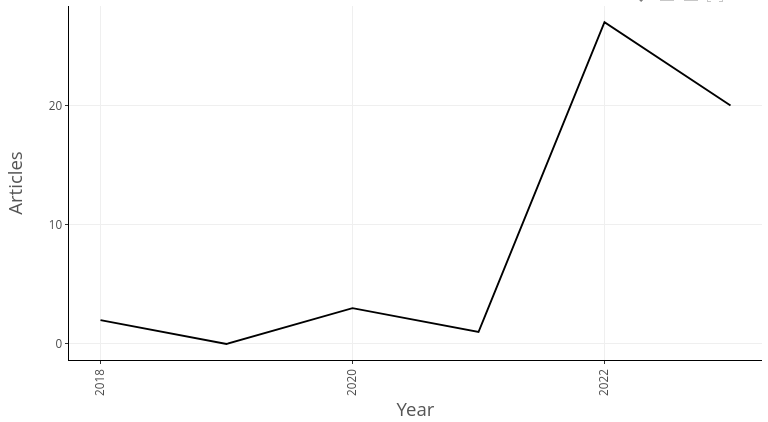
\includegraphics[width=0.8\textwidth]{img/annual_scientific_production}
    %\caption{Annual scientific production.}
    \label{fig:annual_scientific_production}
  \end{figure}
\end{frame}

\begin{frame}
  \frametitle{Average citations per year}
  \begin{figure}
    \centering
    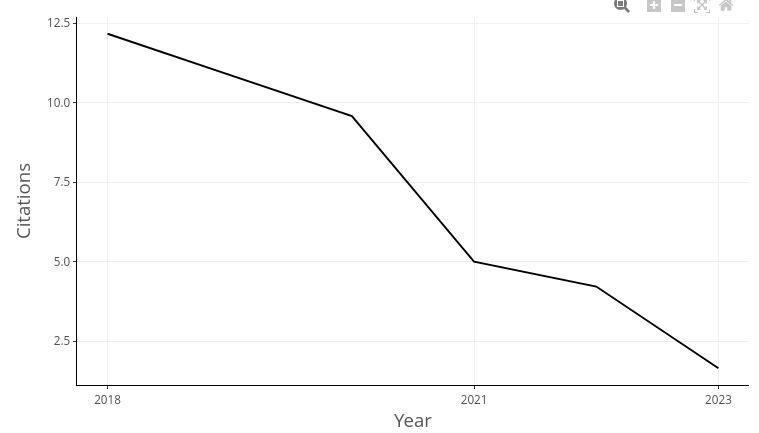
\includegraphics[width=0.8\textwidth]{img/average_citations_per_year}
    %\caption{Average citations per year.}
    \label{fig:average_citations_per_year}
  \end{figure}
\end{frame}

\begin{frame}
  \frametitle{Three fields plot}
  This is an interactive figure (See live). Possible combinations:
  \begin{itemize}
    \item Top keywords, authors, and journals. 
    \item Top authors, references they cite, and keywords they use. 
  \end{itemize}
\end{frame}


\subsection{Sources}

\begin{frame}
  \frametitle{Most relevant sources}
  \begin{figure}
    \centering
    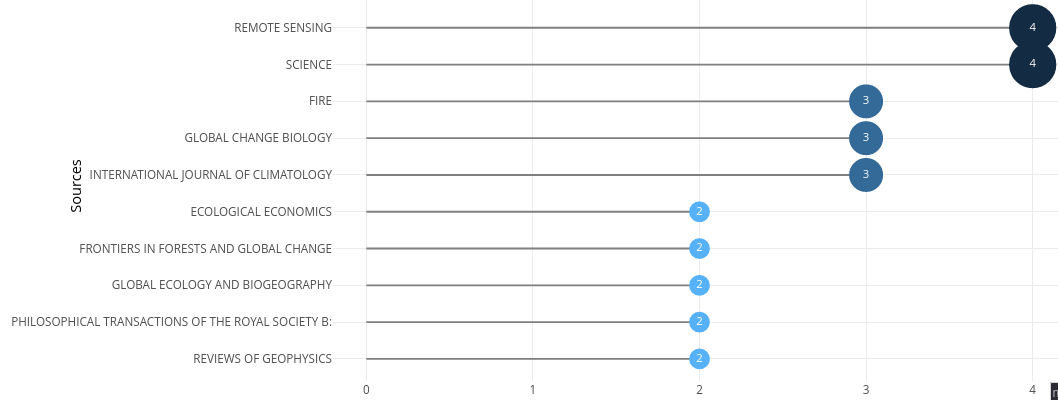
\includegraphics[width=0.8\textwidth]{img/most_relevant_sources.png}
    \caption{A \emph{source} is a journal/book/proceeding/series/etc. which published 
    one or more documents included in the bibliographic collection.} 
    \label{fig:most_relevant_sources}
  \end{figure}
\end{frame}

\begin{frame}
  \frametitle{Most local cited sources}
  \begin{figure}
    \centering
    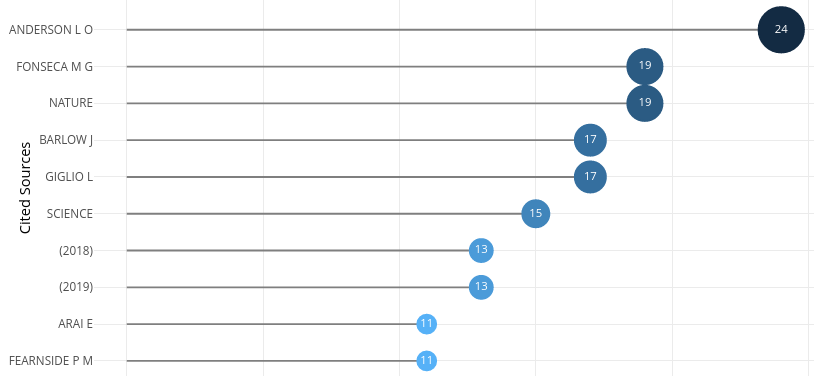
\includegraphics[width=0.8\textwidth]{img/most_local_cited_sources.png}
    \caption{A \emph{cited source} is a journal/book/proceeding/series/etc. 
    included in at least one of the reference list (bibliography) of the 
    document set.}
    \label{fig:most_local_cited_sources}
  \end{figure}
\end{frame}

\begin{frame}
  \frametitle{Bradford's law}
  \begin{figure}
    \centering
    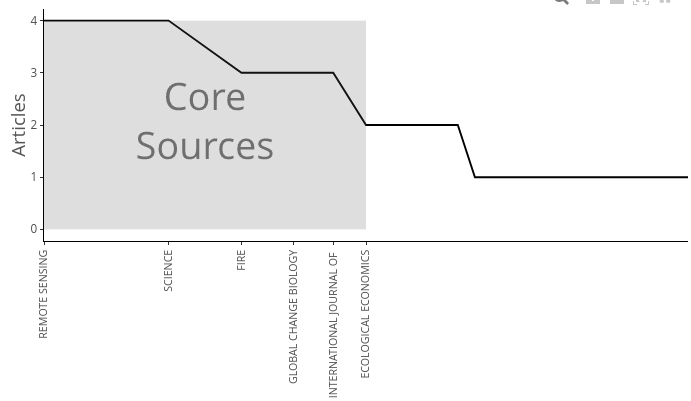
\includegraphics[width=0.8\textwidth]{img/bradfords_law.png}
    \caption{The journals particularly devoted to TreesLab's subjects.}
    \label{fig:bradfords_law}
  \end{figure}
  % If the journals are arranged in descending order of the number of articles 
  % they carried on the subject, then successive zones of periodicals containing
  % the same number of articles on the subject from the simple geometric series
  % $1:n_{s}:n_{s}^2:n_{s}^3$
  % Bradford called the first zone, the nucleus of journals particularly devoted
  % to the given subject.
\end{frame}

\begin{frame}
  \frametitle{Source's local impact}
  \begin{figure}
    \centering
    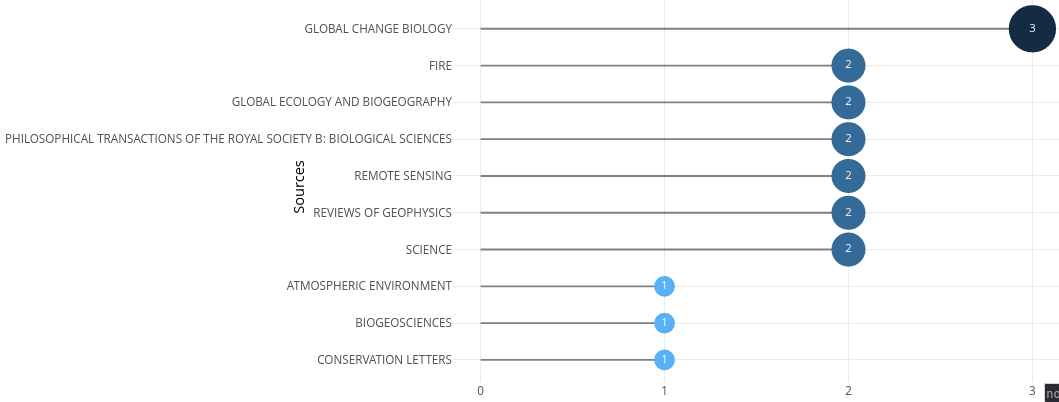
\includegraphics[width=0.8\textwidth]{img/sources_local_impact.png}
    \caption{Impact by H-Index and its generalizations.}
    \label{fig:sources_local_impact}
  \end{figure}
  The Hirsh index (\emph{H-index}) is an author's (or journal's) number of 
  published articles (\emph{h}) each of which has been cited in other papers 
  at least \emph{h} times.
\end{frame}

\begin{frame}
  \frametitle{Sources' production over time}
  \begin{figure}
    \centering
    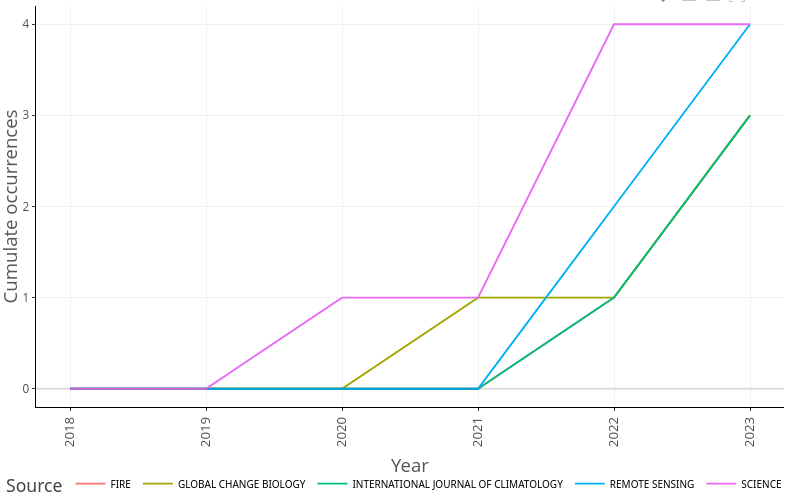
\includegraphics[width=0.8\textwidth]
    {img/sources_production_over_time.png}
    \caption{Number of publications per year.}
    \label{fig:production_over_time}
  \end{figure}
\end{frame}



\subsection{Authors}

\begin{frame}
  \frametitle{Most relevant authors}
  \begin{figure}
    \centering
    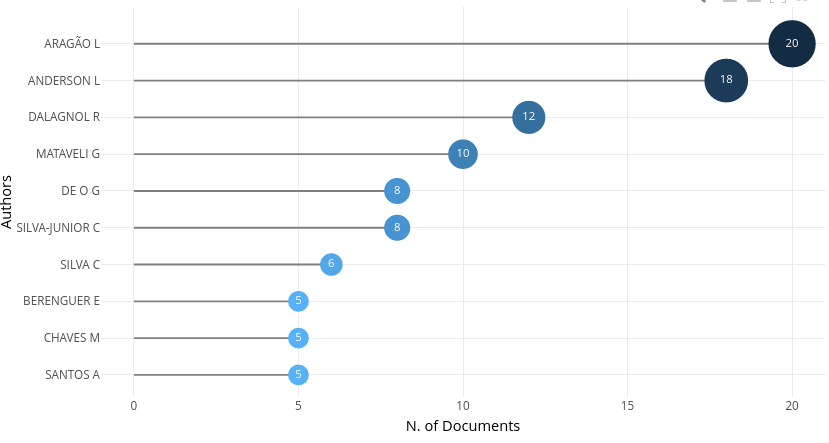
\includegraphics[width=0.8\textwidth]
    {img/most_relevant_authors.png}
    \caption{Most relevant authors (number of documents).}
    \label{fig:most_relevant_authors}
  \end{figure}
\end{frame}

\begin{frame}
  \frametitle{Most relevant authors}
  \begin{figure}
    \centering
    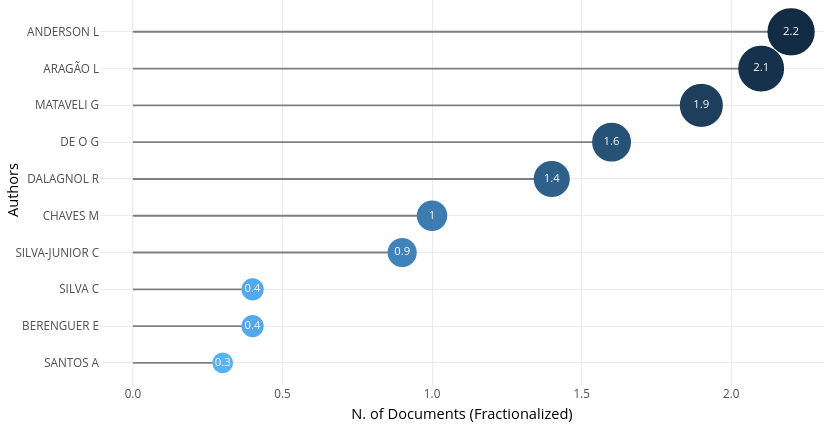
\includegraphics[width=0.7\textwidth]
    {img/most_relevant_authors_fractionalized.png}
    \caption{Most relevant authors (fractionalized).}
    \label{fig:most_relevant_authors_fractionalized}
  \end{figure}
  Fractionalized authorship quantifies an individual author's contributions to 
  a published set of papers (following the hypothesis of uniform contributions
  of all co-authors at each document).
\end{frame}

\begin{frame}
  \frametitle{Author's production over time}
  \begin{figure}
    \centering
    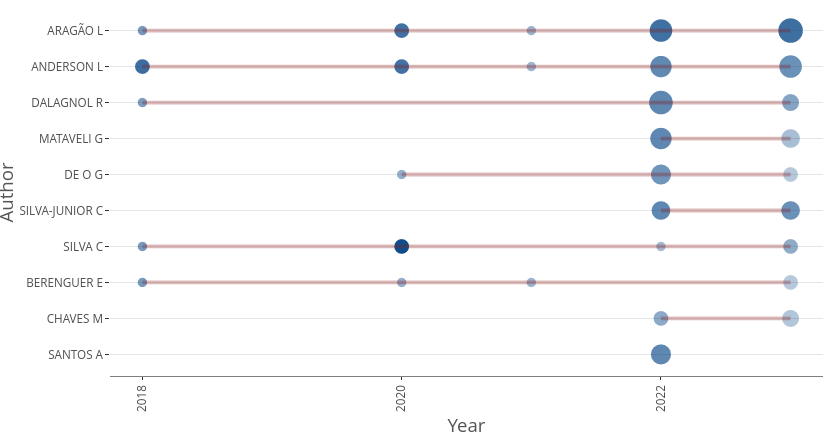
\includegraphics[width=0.7\textwidth]
    {img/authors_production_over_time.png}
    %\caption{Authors production over time}
    \label{fig:authors_production_over_time}
  \end{figure}
  A line represents an author's timeline.
  The buble size is proportional to the number of documents. 
  The color intensity is proportional to the total citations per year.
\end{frame}

\begin{frame}
  \frametitle{Author productivity through Lotka's law}
  \begin{figure}
    \centering
    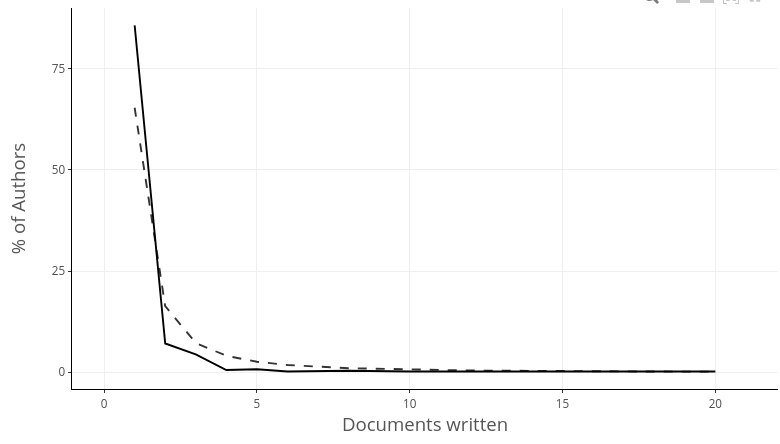
\includegraphics[width=0.6\textwidth]
    {img/loktas_law.png}
    \caption{Dashed line represents the theoretical distribution.}
    \label{fig:loktas_law}
  \end{figure}
  \emph{As the number of articles published increases, authors producing that
  many publications become less frequent.}
\end{frame}

\begin{frame}
  \frametitle{Authors' local impact}
  \begin{figure}
    \centering
    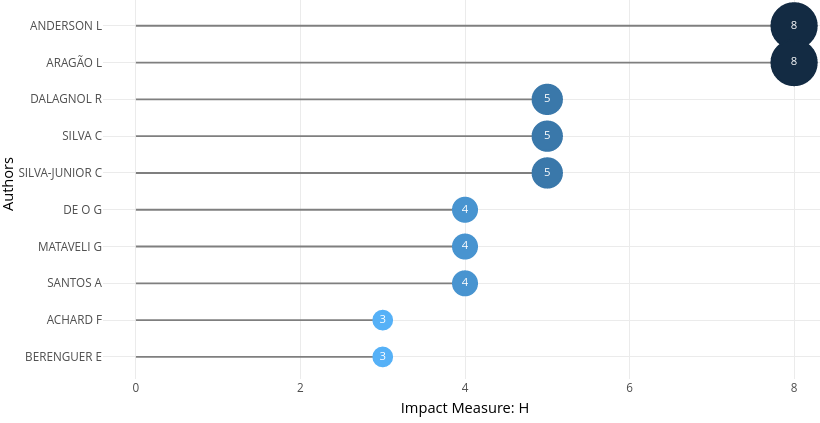
\includegraphics[width=0.8\textwidth]
    {img/authors_local_impact.png}
    \caption{Authors' local impact by H-index and its generalizations.}
    \label{fig:authors_local_impact}
  \end{figure}
\end{frame}

\begin{frame}
  \frametitle{Most relevant affiliations}
  \begin{figure}
    \centering
    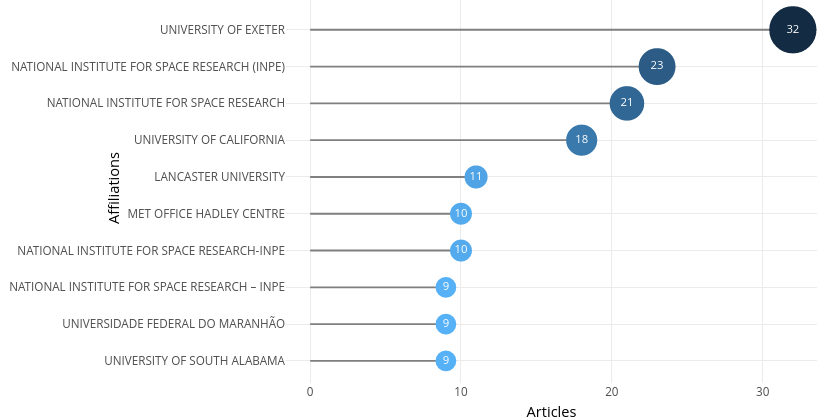
\includegraphics[width=0.8\textwidth]
    {img/most_relevant_affiliations.png}
    \caption{INPE's affiliation strings need cleaning!}
    \label{fig:most_relevant_affiliations}
  \end{figure}
\end{frame}

% \begin{frame}
%   \frametitle{Corresponding authors' country}
%   NOTE: biblioshiny is throwing an error!
% \end{frame}

\begin{frame}
  \frametitle{Countries' scientific production}
  \begin{figure}
    \centering
    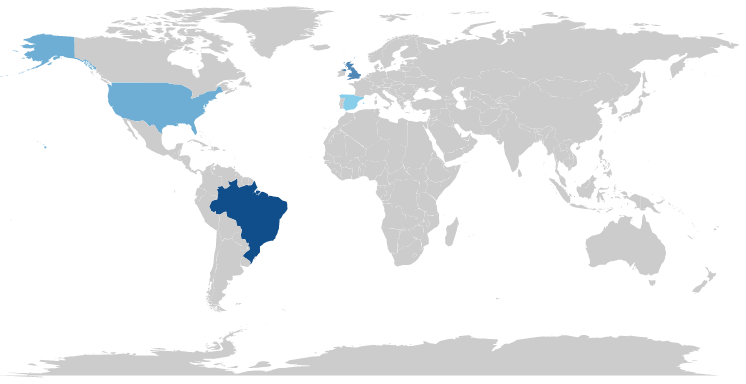
\includegraphics[width=0.8\textwidth]
    {img/countries_scientific_production.png}
    \caption{The color intensity is proportional to the number of publications.}
    \label{fig:countries_scientific_production}
  \end{figure}
\end{frame}

\begin{frame}
  \frametitle{Most cited countries}
  \begin{figure}
    \centering
    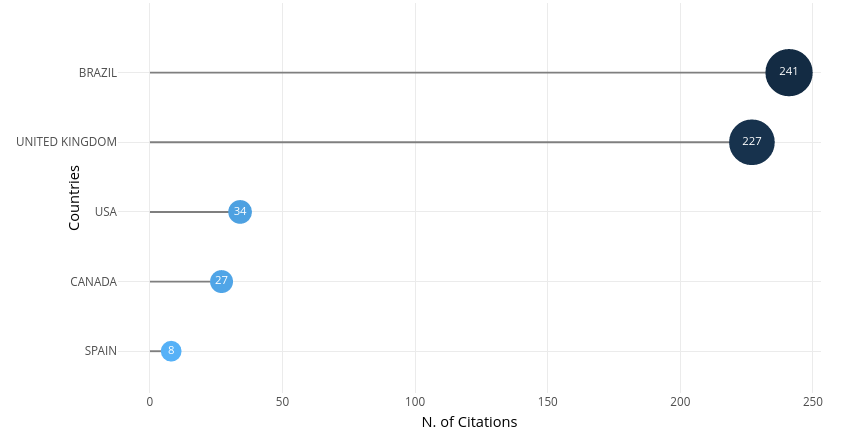
\includegraphics[width=0.8\textwidth]
    {img/most_cited_countries.png}
    %\caption{Most cited countries.}
    \label{fig:most_cited_countries}
  \end{figure}
\end{frame}



\subsection{Documents}

\begin{frame}
  \frametitle{Documents and references}
  \begin{itemize}
    \item \emph{Document (or citing document)}: Scientific document (article, 
      review, conference proceeding, etc.) included in a bibliographic 
      collection.
    \item \emph{Reference (or cited reference)}: Scientific document included 
      in at least one of the reference lists (bibliography) of the document 
      set. Then "a reference is cited by one or more documents".
    \item \emph{Cited document}: Scientific document included in a 
      bibliographic collection and, at the same time, it is cited in at least
      one other document in the collection. Cited documents are a subset of the
      reference set.
  \end{itemize}
\end{frame}

\begin{frame}
  \frametitle{Global and local citations}
  \begin{columns}
    \begin{column}{0.5\textwidth}
      Global citations.
      \begin{itemize}
        \item Measures the number of citations a document has received from 
          documents contained in the entire database (e.g. WoS or Scopus).
        \item Measures the impact of a document in the whole bibliographic 
          database.
        \item For many documents, a large part of global citations could come 
          from other disciplines!
      \end{itemize}
    \end{column}
    \begin{column}{0.5\textwidth}
      Local citations.
      \begin{itemize}
        \item Measures the number of citations a document has received from 
          documents included in the analyzed collection. 
        \item Is calculated analyzing the whole reference set. 
        \item Measures the impact of a document in the analyzed collection.
      \end{itemize}
    \end{column}
  \end{columns}
\end{frame}

\begin{frame}
  \frametitle{Most global cited documents}
  \begin{figure}
    \centering
    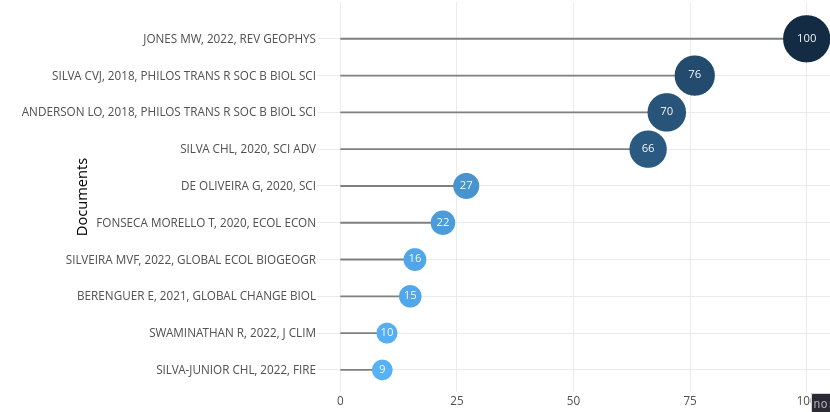
\includegraphics[width=0.8\textwidth]
    {img/most_global_cited_documents.png}
    \caption{Is there an impactful paper?}
    \label{fig:most_global_cited_documents}
  \end{figure}
\end{frame}

% \begin{frame}
%   \frametitle{Most local cited documents}
%   Bibmetrix throws an error!
% \end{frame}

\begin{frame}
  \frametitle{Reference publication year spectroscopy}
  \begin{figure}
    \centering
    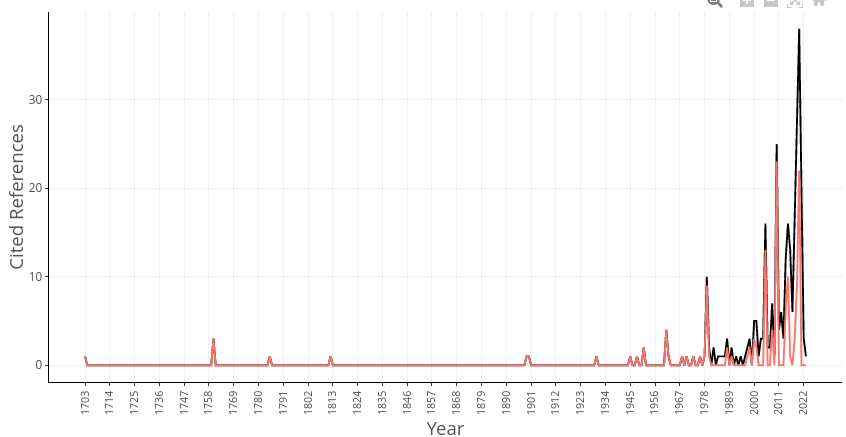
\includegraphics[width=0.8\textwidth]
    {img/references_spectroscopy.png}
    \caption{Number of cited references per year and deviation from the 5-year
    mean.}
    \label{fig:references_spectroscopy}
  \end{figure}
  %Identify the historical origins of a research field.
\end{frame}

\begin{frame}
  \frametitle{Most frequent words (Keywords Plus)}
  \begin{figure}
    \centering
    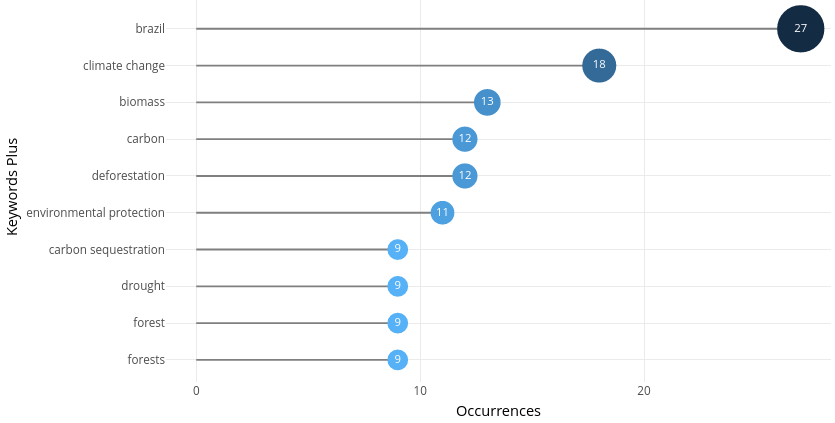
\includegraphics[width=0.8\textwidth]
    {img/most_frequent_words_keywords_plus.png}
    %\caption{Most frequent words (Keywords Plus).}
    \label{fig:most_frequent_words_keywords_plus}
  \end{figure}
  \emph{Keywords Plus} are words or phrases that appear frequently in the 
  titles of an article's references and not necessarily in the title of the 
  article or as Author Keywords.
\end{frame}

\begin{frame}
  \frametitle{Most frequent words (Author's keywords)}
  \begin{figure}
    \centering
    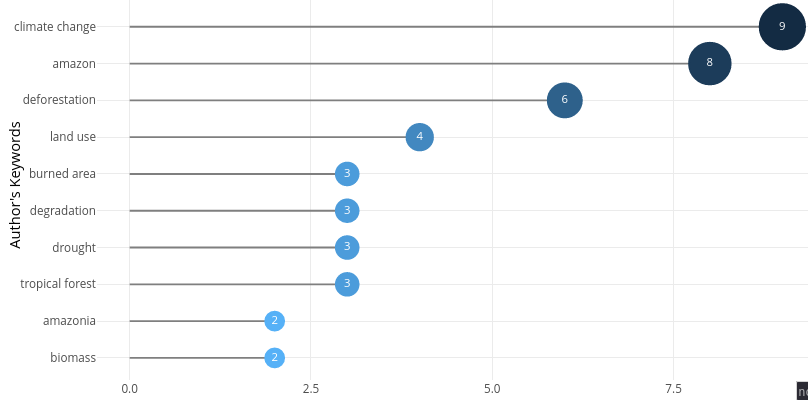
\includegraphics[width=0.8\textwidth]
    {img/most_frequent_words_authors_keywords.png}
    %\caption{Most frequent words (Author's keywords).}
    \label{fig:most_frequent_words_authors_keywords}
  \end{figure}
  \emph{Authors' Keywords} are the terms the authors believe best represent
  the content of their papers. Beware of plurals and conjugations.
\end{frame}

\begin{frame}
  \frametitle{Most frequent words (titles' words)}
  \begin{figure}
    \centering
    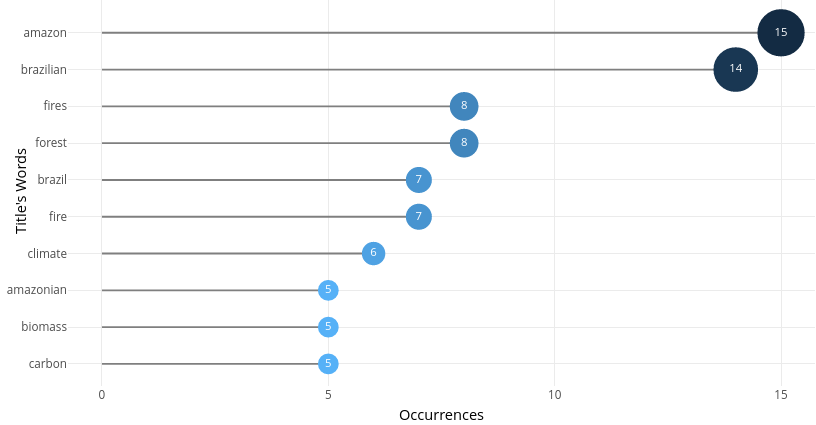
\includegraphics[width=0.8\textwidth]
    {img/most_frequent_words_titles_words.png}
    %\caption{Most frequent words (titles' words).}
    \label{fig:most_frequent_words_titles_words}
  \end{figure}
  Words extracted from titles (or abstracts) removing "stop words" and 
  punctuation.
\end{frame}

\begin{frame}
  \frametitle{Most frequent words (abstracts' words)}
  \begin{figure}
    \centering
    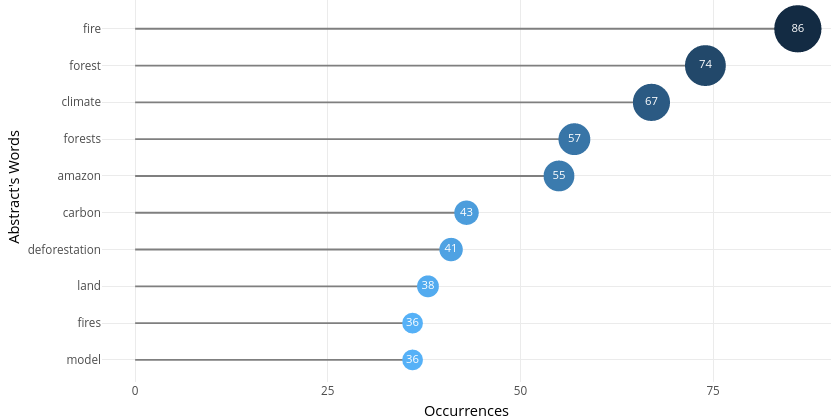
\includegraphics[width=0.8\textwidth]
    {img/most_frequent_words_abstracts_words.png}
    %\caption{Most frequent words (abstracts' words).}
    \label{fig:most_frequent_words_abstracts_words}
  \end{figure}
  Abstract words need to be cleaned to avoid trivial terms such as "paper", 
  "study", "work", "data", etc.
\end{frame}

\begin{frame}
  \frametitle{Wordclouds}
  \begin{figure}
    \centering
    \begin{subfigure}{0.4\textwidth}
      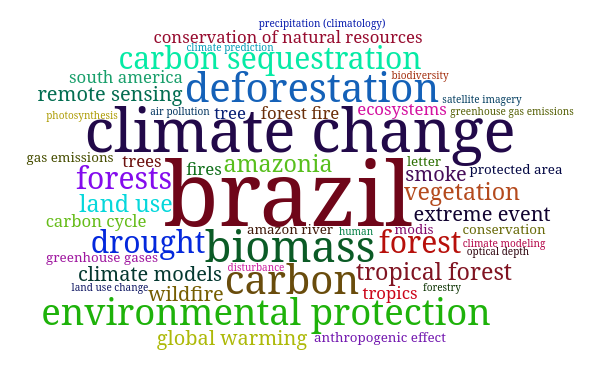
\includegraphics[width=0.8\textwidth]
      {img/wordcloud_keywords_plus.png}
      \caption{Keywords Plus}
      \label{fig:wordcloud_keywords_plus} 
    \end{subfigure}
    \begin{subfigure}{0.4\textwidth}
      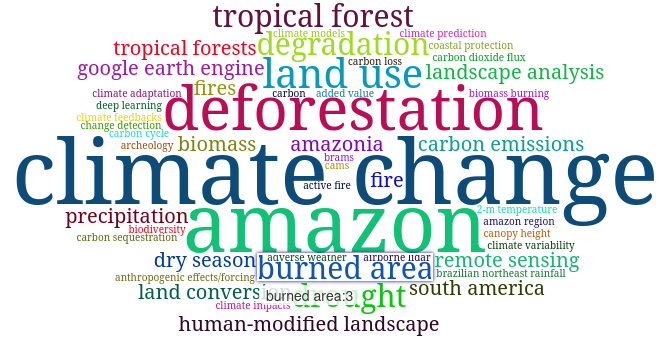
\includegraphics[width=0.8\textwidth]
      {img/wordcloud_authors_keywords.png}
      \caption{Authors' Keywords}
      \label{fig:wordcloud_authors_keywords} 
    \end{subfigure}
    \begin{subfigure}{0.4\textwidth}
      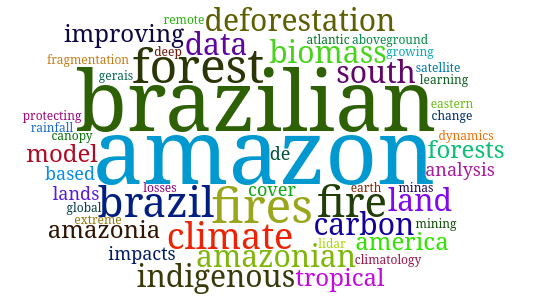
\includegraphics[width=0.8\textwidth]
      {img/wordcloud_titles_words.png}
      \caption{Titles' words.}
      \label{fig:wordcloud_titles_words} 
    \end{subfigure}
    \begin{subfigure}{0.4\textwidth}
      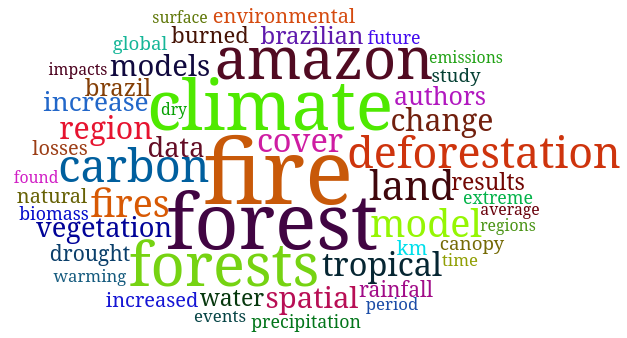
\includegraphics[width=0.8\textwidth]
      {img/wordcloud_abstracts_words.png}
      \caption{Abstracts' words.}
      \label{fig:wordcloud_abstract_words} 
    \end{subfigure}
  \end{figure}
\end{frame}

\begin{frame}
  \frametitle{Treemaps}
  \begin{figure}
    \centering
    \begin{subfigure}{0.45\textwidth}
      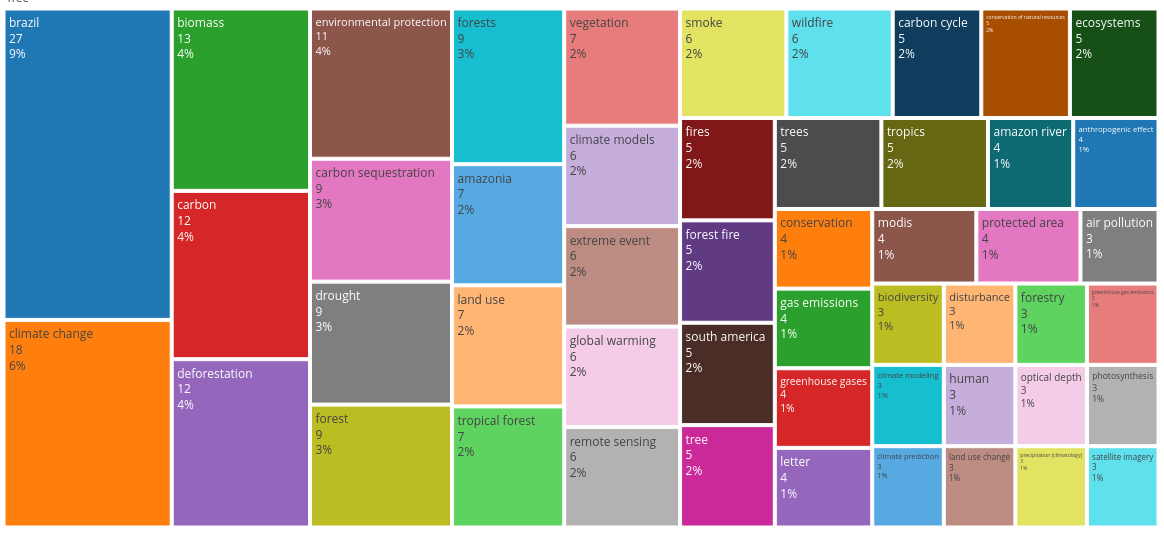
\includegraphics[width=0.99\textwidth]
      {img/treemap_keywords_plus.png}
      \caption{Keywords Plus}
      \label{fig:treemap_keywords_plus} 
    \end{subfigure}
    \begin{subfigure}{0.45\textwidth}
      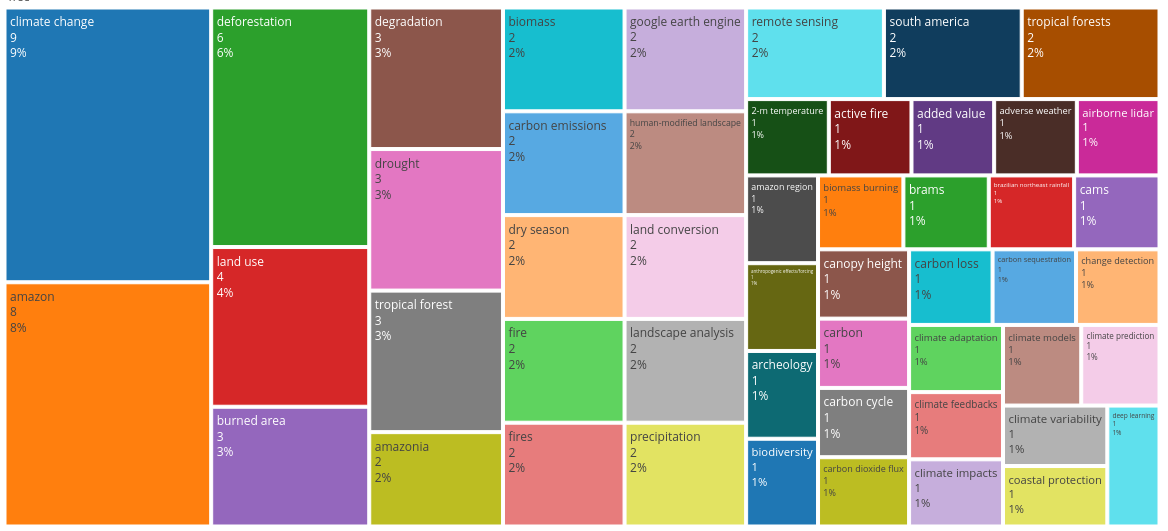
\includegraphics[width=0.99\textwidth]
      {img/treemap_authors_keywords.png}
      \caption{Authors' Keywords}
      \label{fig:treemap_authors_keywords} 
    \end{subfigure}
    \begin{subfigure}{0.45\linewidth}
      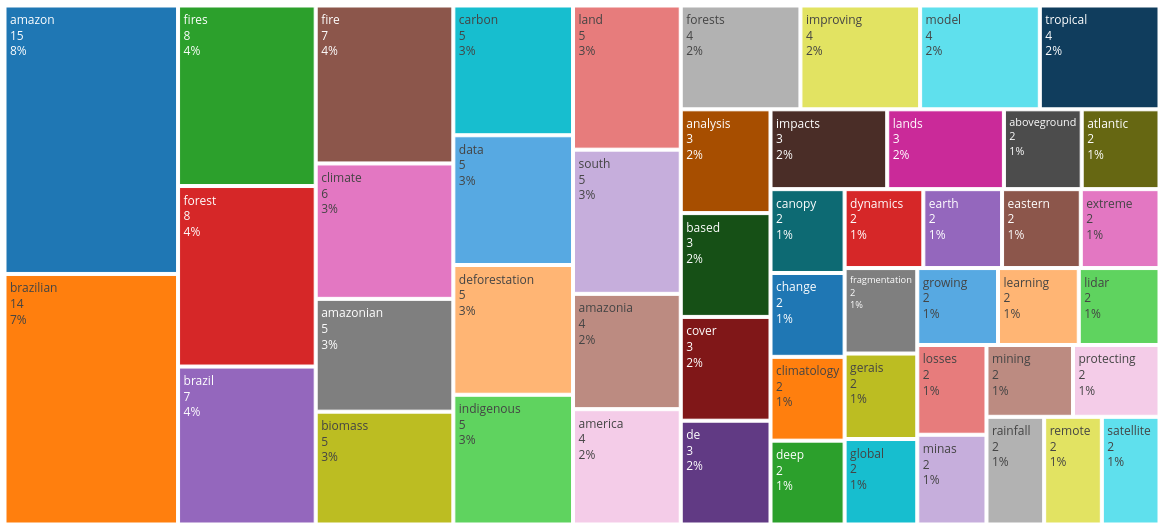
\includegraphics[width=0.99\textwidth]
      {img/treemap_titles_words.png}
      \caption{Titles' words.}
      \label{fig:treemap_titles_words} 
    \end{subfigure}
    \begin{subfigure}{0.45\linewidth}
      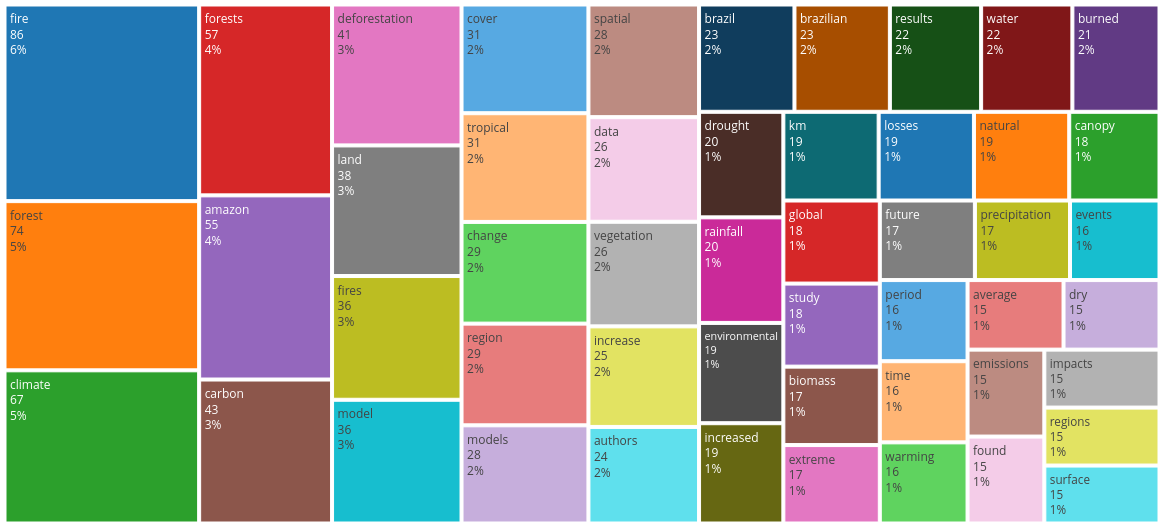
\includegraphics[width=0.99\textwidth]
      {img/treemap_abstracts_words.png}
      \caption{Abstracts' words.}
      \label{fig:treemap_abstract_words} 
    \end{subfigure}
  \end{figure}
\end{frame}

\begin{frame}
  \frametitle{Words' frequency over time}
  \begin{figure}
    \centering
    \begin{subfigure}{0.4\textwidth}
      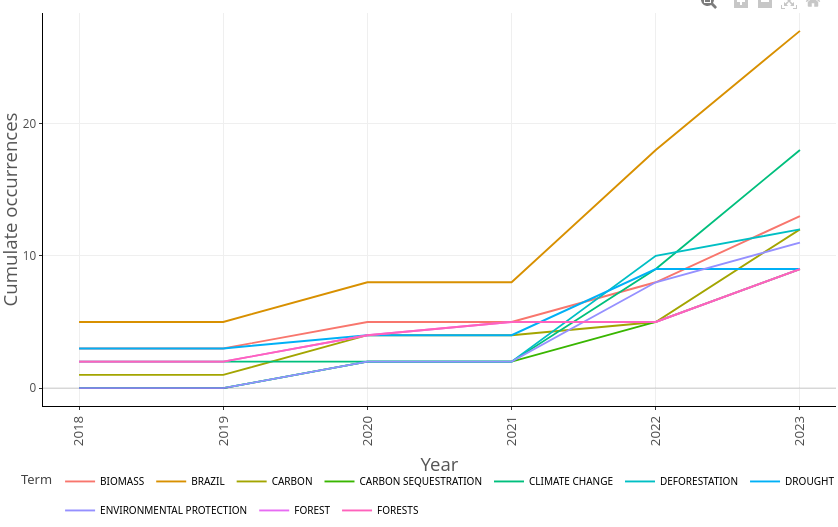
\includegraphics[width=0.8\textwidth]
      {img/words_frequency_over_time_keywords_plus.png}
      \caption{Keywords Plus}
      \label{fig:wordcloud_keywords_plus} 
    \end{subfigure}
    \begin{subfigure}{0.4\textwidth}
      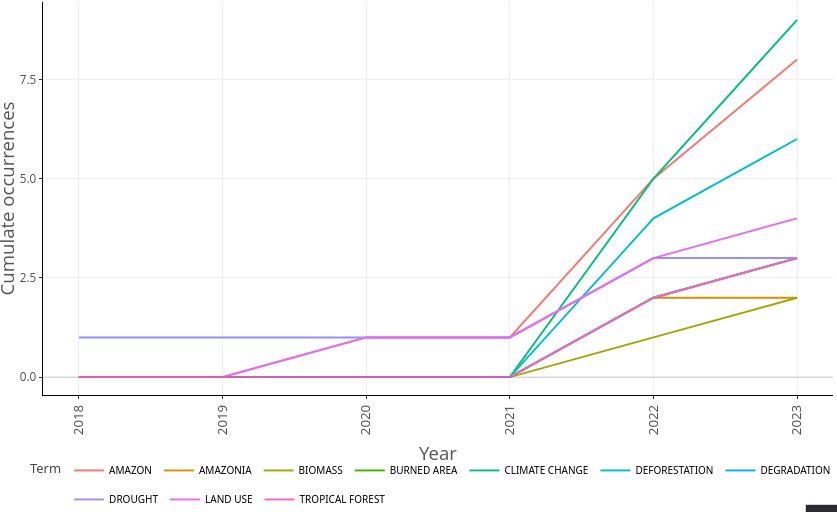
\includegraphics[width=0.8\textwidth]
      {img/words_frequency_over_time_authors_keywords.png}
      \caption{Authors' Keywords}
      \label{fig:wordcloud_authors_keywords} 
    \end{subfigure}
    \begin{subfigure}{0.4\textwidth}
      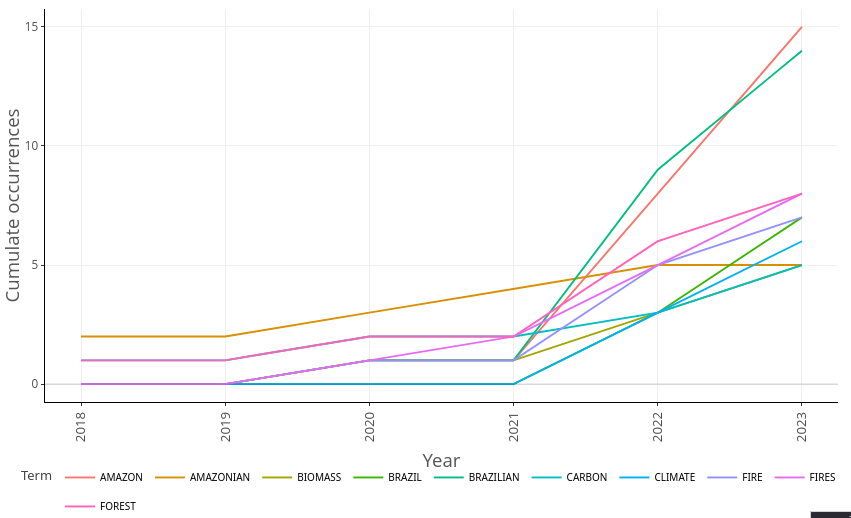
\includegraphics[width=0.8\textwidth]
      {img/words_frequency_over_time_titles_words.png}
      \caption{Titles' words.}
      \label{fig:wordcloud_titles_words} 
    \end{subfigure}
    \begin{subfigure}{0.4\textwidth}
      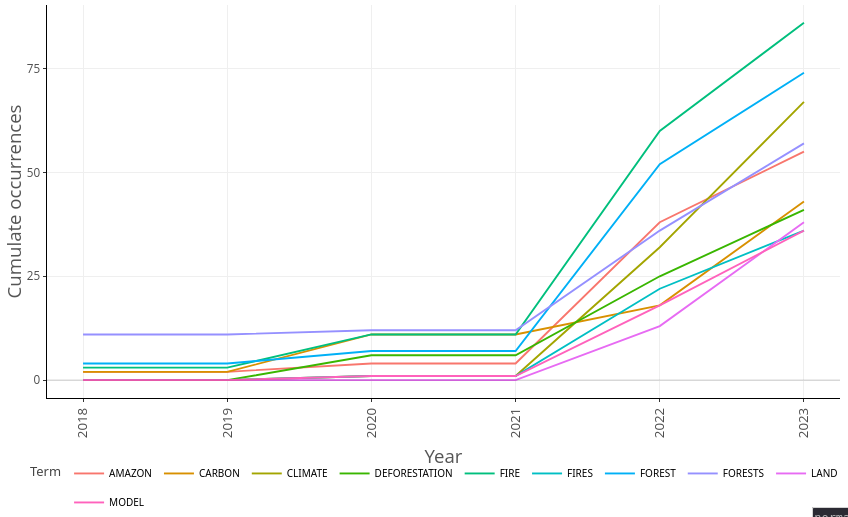
\includegraphics[width=0.8\textwidth]
      {img/words_frequency_over_time_abstracts_words.png}
      \caption{Abstracts' words.}
      \label{fig:wordcloud_abstract_words} 
    \end{subfigure}
  \end{figure}
\end{frame}



\section{Knowledge synthesis}

\begin{frame}
  \frametitle{Structures of knowledge}
  \begin{itemize}
    \item \emph{Conceptual}: What science talks about. 
    \item \emph{Intellectual}: How the work of an author influences a given 
      scientific community. 
    \item \emph{Social}: How authors, institutions, and countries interact each
      other.
  \end{itemize}
  \emph{Science mapping} allows investigating scientific knowledge from a 
  statistical point of view.
\end{frame}

% TODO: https://bibliometrix.org/biblioshiny/assets/player/KeynoteDHTMLPlayer.html#93

\subsection{Conceptual structure}
\subsection{Intellectual structure}
\subsection{Social structure}




\section{Summary}

\begin{frame}
  \frametitle{Take home message}
  \begin{itemize}
    \item TODO.
  \end{itemize}
\end{frame}

\begin{frame}[allowframebreaks]
  \frametitle{References}
  %\bibliographystyle{amsalpha}
  \bibliographystyle{plainnat}
  \bibliography{slides.bib}
\end{frame}

\begin{frame}
  \frametitle{Queries}
  Queries for TreesLab's papers.
\end{frame}

\begin{frame}[allowframebreaks]
  \frametitle{Query Scopus}
  \inputsql{code/query_scopus.txt}
\end{frame}

\begin{frame}[allowframebreaks]
  \frametitle{Query WoS}
  \inputsql{code/query_wos.txt}
\end{frame}

\end{document}

